\documentclass{beamer}


\mode<presentation>
{
\usetheme{default}
\usecolortheme{default}
\usefonttheme{default}
\setbeamertemplate{navigation symbols}{}
\setbeamertemplate{caption}[numbered]
}
\usepackage{caption}
\usepackage[english]{babel}
\usepackage[utf8x]{inputenc}
\usepackage{graphicx}
\usepackage{verbatim}
\usepackage{physics}
\usepackage{amsmath}
\newcommand\norm[1]{\left\lVert#1\right\rVert}

\makeatletter
\renewcommand\footnotesize{%
\@setfontsize\footnotesize\@ixpt{6}%
\abovedisplayskip 8\p@ \@plus2\p@ \@minus4\p@
\abovedisplayshortskip \z@ \@plus\p@
\belowdisplayshortskip 4\p@ \@plus2\p@ \@minus2\p@
\def\@listi{\leftmargin\leftmargini
\topsep 4\p@ \@plus2\p@ \@minus2\p@
\parsep 2\p@ \@plus\p@ \@minus\p@
\itemsep \parsep}%
\belowdisplayskip \abovedisplayskip
}
\makeatother

\title[Your Short Title]{Magneto-static Analysis of a Brushless DC Motor}
\author{\small Tom Ginsberg, Brendan Posehn}
\date{}

\begin{document}

    \begin{frame}
        \vspace{0.5cm}
        \titlepage
        \vspace{-1.5cm}
        \begin{center}
            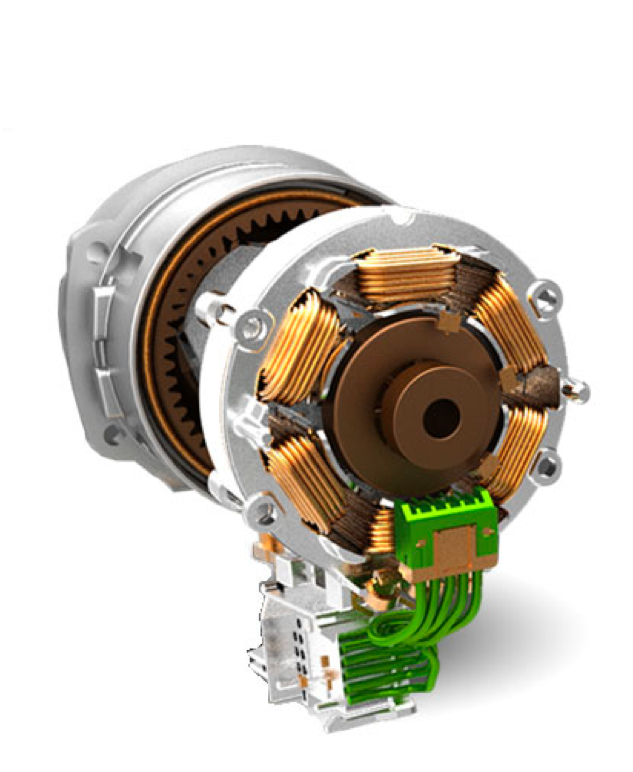
\includegraphics[width=2in]{render.png}
        \end{center}
    \end{frame}

    \begin{frame}{Overview}
        \begin{itemize}
            \item {\large Background}\\
            Brushless DC Motors
            \item {\large Theory}\\
            Magneto-statics, Permanent Magnets, Non Linear Materials, Non Linear FEM
            \item {\large Implementation}\\
            Meshing, Matrix Assembly, Solvers, BLDC Problem
            \item {\large Results}\\
            Diagrams, Torques
        \end{itemize}

    \end{frame}
    \begin{frame}{Theory: Magnetostatics in a 2D Cross Section}
        If current is only perpendicular to the 2D plane, then
        \begin{align*}
            &\nabla\times \nu B=J\text{ and }\nabla \times A = B\\
            &\nabla\times \nu \nabla\times A=J \iff \nabla\cdot \nu \nabla A=J
        \end{align*}
        \begin{center}
            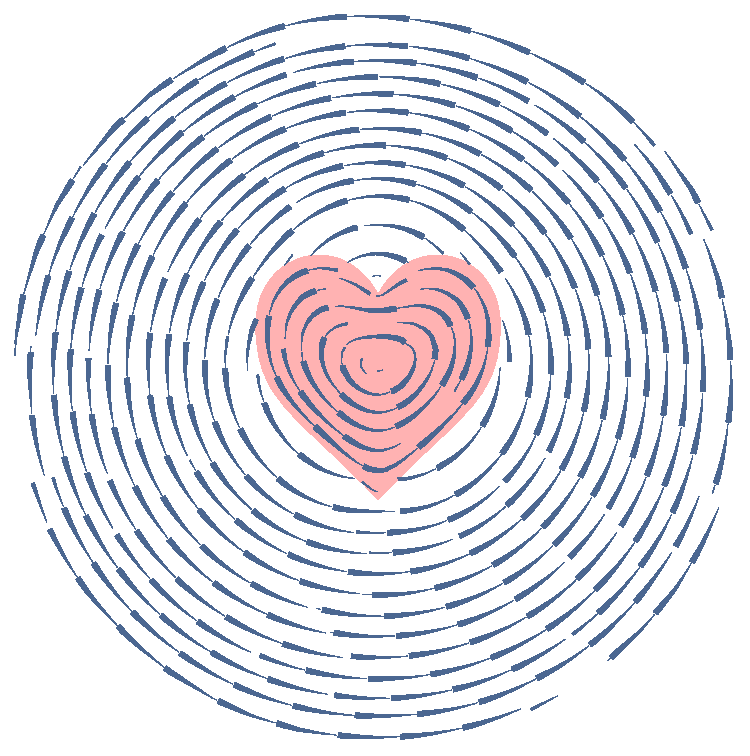
\includegraphics[width=3in]{heartwire.pdf}
        \end{center}
    \end{frame}
    \begin{frame}{Theory: Permanent Magnets}
        Maxwell's Equation's for Permanent Magnets
        \begin{align*}
            B &= \mu H +\mu_0 M_r\text{ and } \nabla \times H = J \implies \nabla \times \nu B=J+\nabla\times \nu\mu_0 M_r\\
            J_m&\triangleq \nabla\times \nu\mu_0 M_r \implies \nabla \times \nu B=J+J_m
        \end{align*}
        \begin{center}
            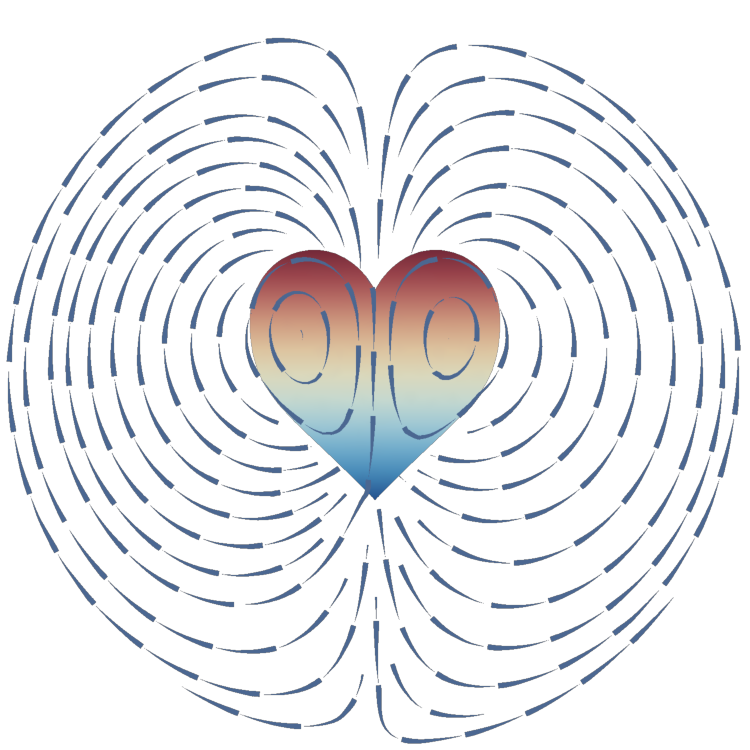
\includegraphics[width=3in]{heartmag.pdf}
        \end{center}
    \end{frame}
    \begin{frame}{Permenant Magnets}
        We use a \textit{2D-coil} model for permanent magnets.
        \begin{itemize}
            \item \textbf{Assumption}: A bar magnet has a similar field to a current carrying coil
            \item \textbf{Heuristic}: Any magnet geometry can be approximated from gluing together curved bar magnets
        \end{itemize}
        \begin{center}
            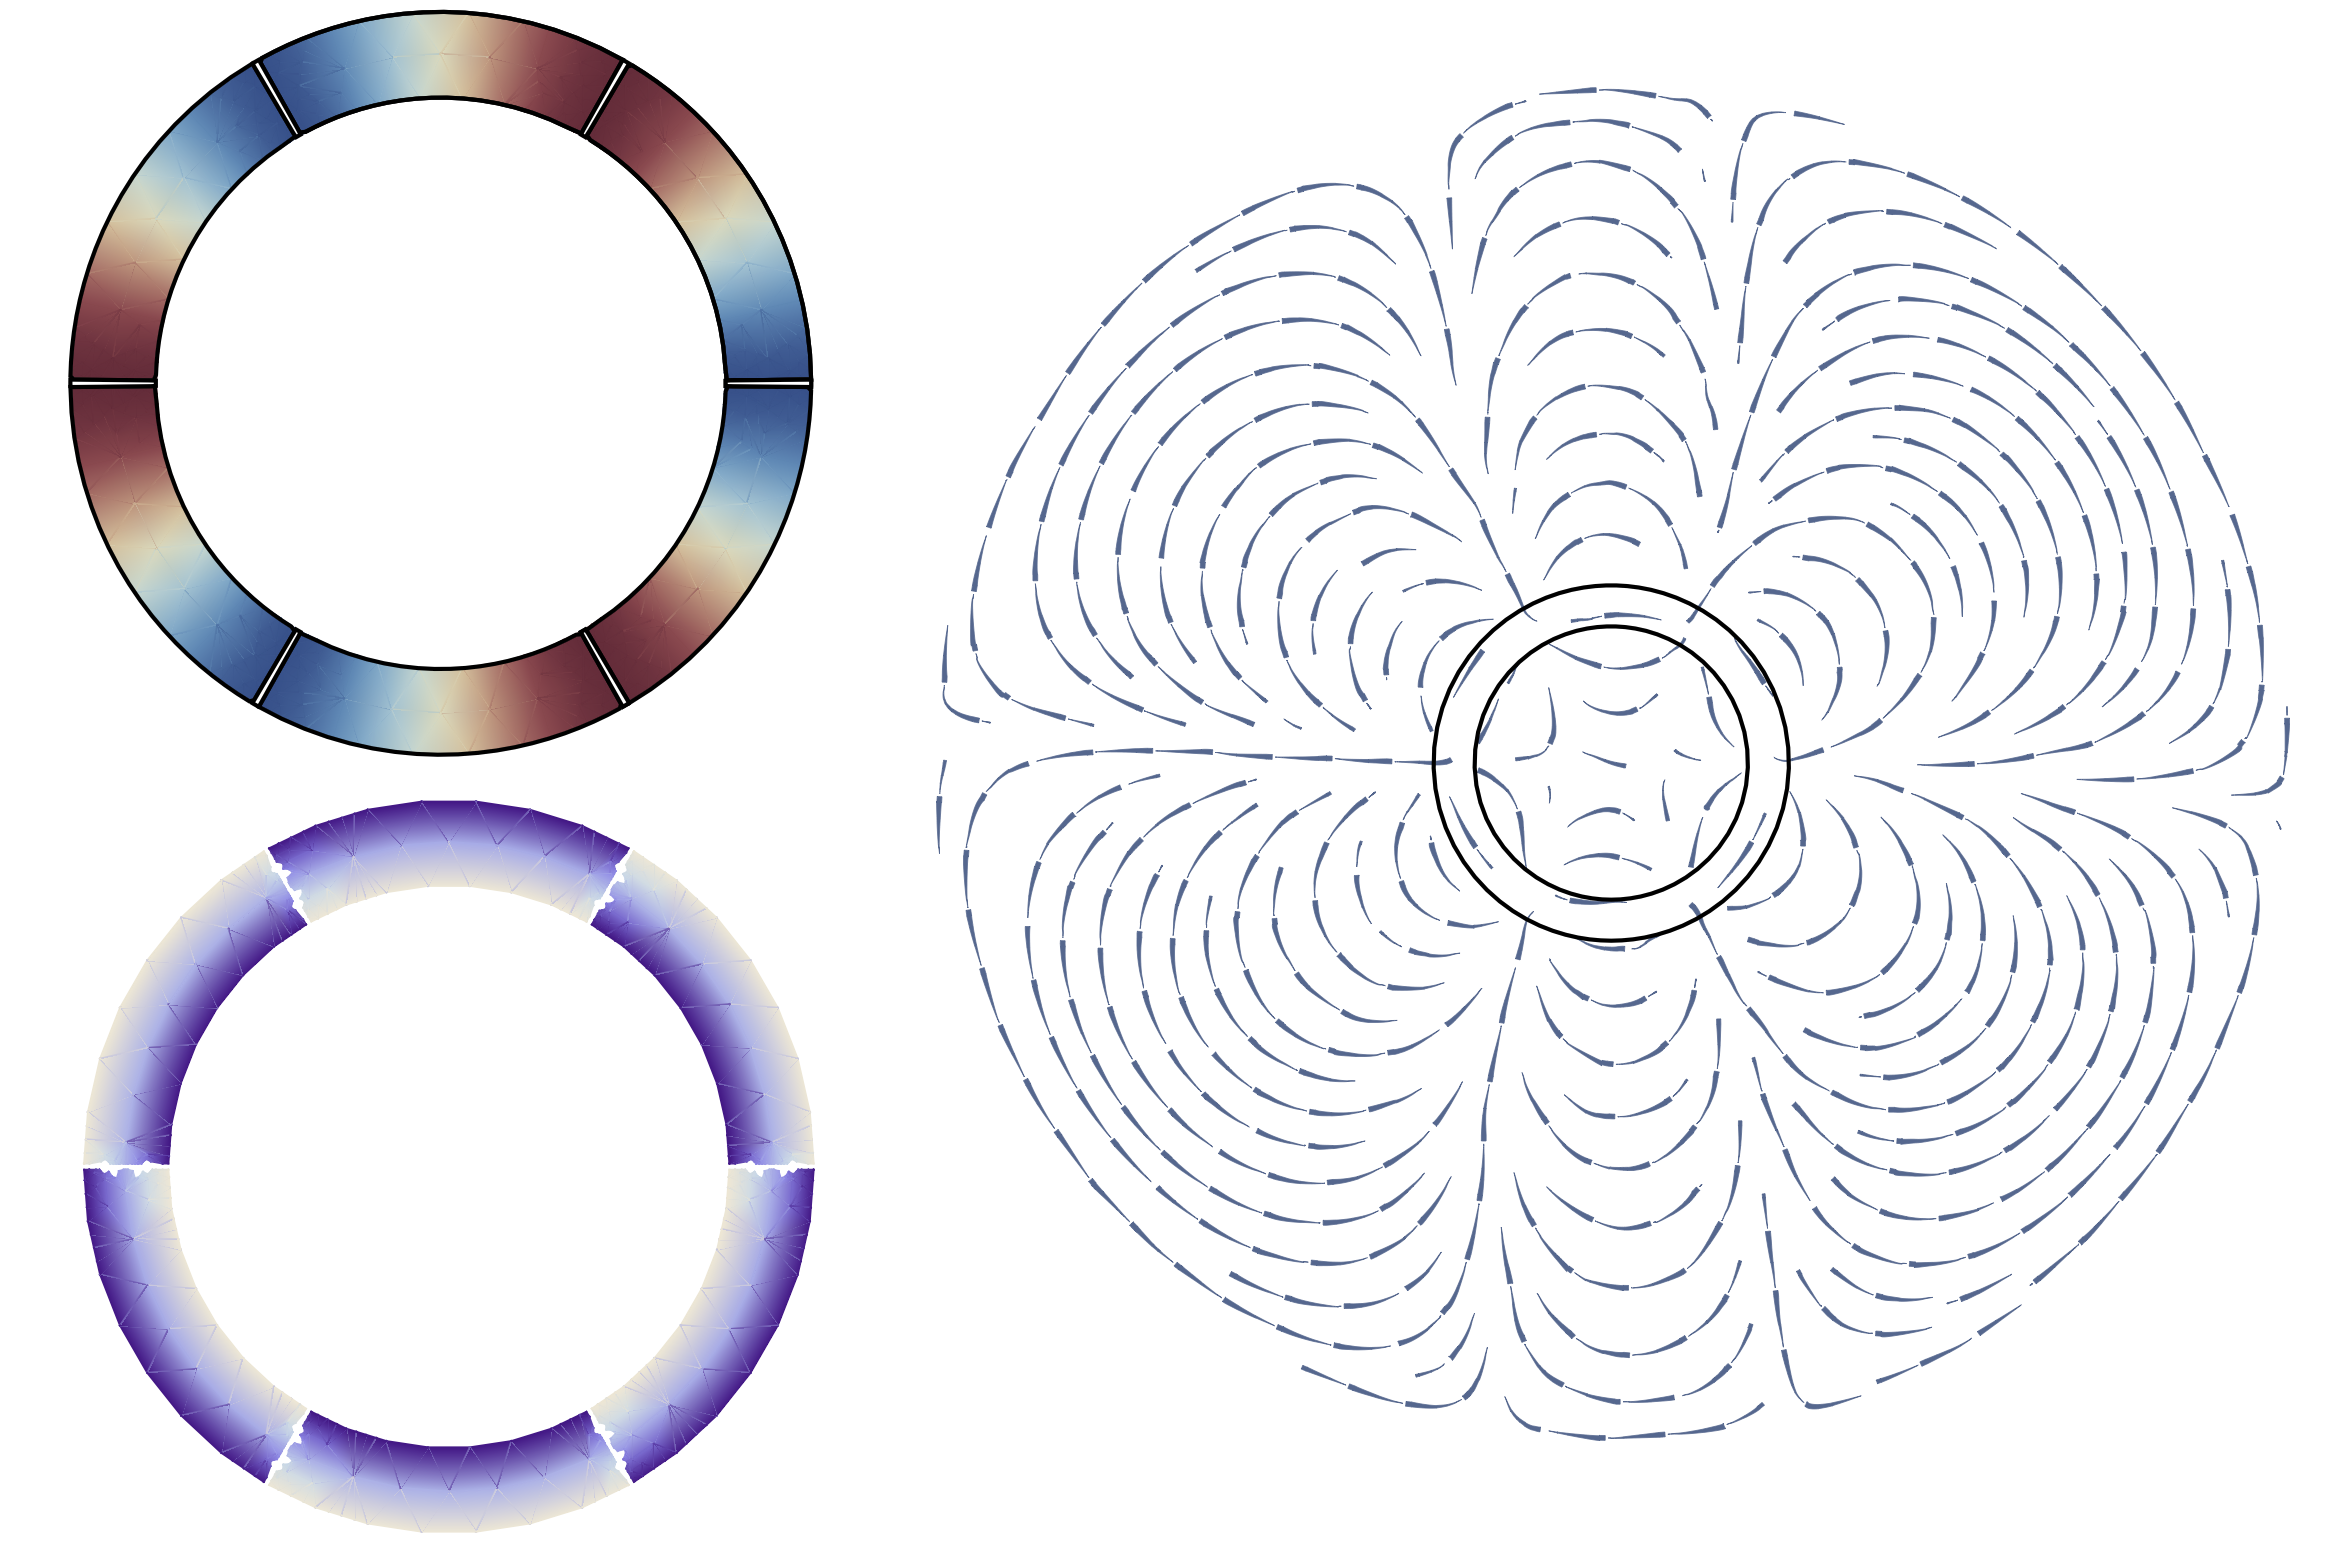
\includegraphics[width=3in]{ring.png}
        \end{center}
    \end{frame}
    \begin{frame}{Theory: Non Linear FEM}
        How can we use FEM to solve problems in the form of
        \[\nabla\cdot\left(\alpha(\|\nabla\phi\|)*\nabla\phi\right)=f(x,y)\]
        \textbf{First thing}: Determine $\|\nabla\phi\|$ on a single element in terms of node values of $\phi$: $\phi^{e}:=\left( \phi_i, \phi_j, \phi_k \right)^{\text{T}}$
        \begin{gather*}
            \norm{\left(\pdv{\phi}{x},\pdv{\phi}{y}\right)}=\norm{\left(\pdv{\vec{N}}{x}, \pdv{\vec{N}}{y} \right)^{\text{T}}\cdot \phi^{e}}\\
            \hat{\alpha}(\phi^e):=\alpha(\norm{\nabla\phi})
        \end{gather*}
    \end{frame}
    \begin{frame}{Solving the Non Linear System}
        Now our element matrix equation looks like:
        \[F_e(\phi^{e})=\mathbf{K}^e\cdot \phi^e*\hat{\alpha}(\phi^{e})-\vec{b}^e=0\]
        No more linear solver :( we need to use Newton's Method\\
        \smallbreak
        Consider the vector equation $f(\vec{x})=0$
        \begin{itemize}
            \item Start with the guess $\vec{x}\approx\vec{x}_0$
            \item Expand in power series
            \[f(\vec{x})\approx f(\vec{x}_0)+\mathbf{J}_{f(\vec{x}_0)}(\vec{x}-\vec{x}_0)\approx 0\]
            \item Solve a linear system for $\vec{x_0}$ to find a better guess for $\vec{x}$.
            Iterate.
            \begin{align*}
                &\mathbf{J}_{f(\vec{x}_n)}\left(\vec{x}_{n}-\vec{x}_{n+1}\right)=f(\vec{x}_{n})\\
                &\mathbf{J}_{F_e(\phi_n^e)}=\mathbf{K}^e\left( \mathbf{I}*\hat{\alpha}(\phi_n^e)+\left(\phi_n^e\right)\cdot \nabla^{\text{T}}\hat{\alpha}(\phi_n^e) \right)\\
            \end{align*}
        \end{itemize}
    \end{frame}
    \begin{frame}{Implementation: FEA\textit{lite}}
        \hspace{-0.72cm}
        
\includegraphics[width=4.5in]{technology.pdf}

    \end{frame}


    \begin{frame}{Mesh}
        \begin{itemize}
            \item Generated with Mathematica
            \item Triangular Elements
            \item Linear Shape Functions
            $A=\sum_{i=1}^{3}N_{i}A_i$
        \end{itemize}
        \begin{center}
            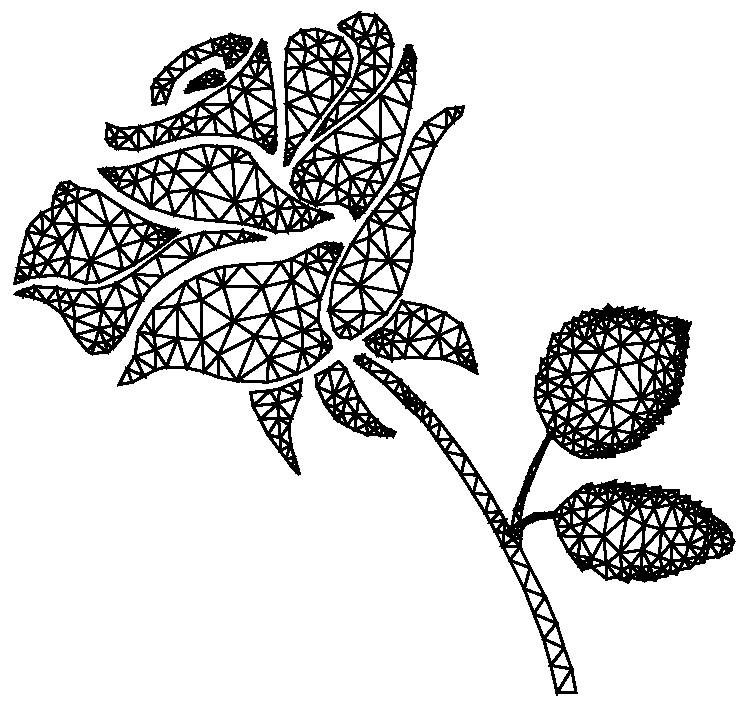
\includegraphics[width=2.8in]{rosemesh.pdf}
        \end{center}
    \end{frame}
    \begin{frame}[fragile]
        \frametitle{Matrix Assembly}
        Dense element matrices are assembled into a sparse global matrix using by substituting equality constraints at shared nodes
        \[\mathbf{K}_{i,j}=\sum_{e\in E(i,j)}\sum_{k=l=0}^{3} \mathbf{K}^{e}_{k,l}*\alpha(e)\]
        $e=\{v_a,v_b,v_c\}$ is an element, $E$ is the element set, $E(i,j)$ is the set of elements $\{\,e\,|\,e\in E,\,\left(\{v_i\}\cup\{v_j\}\right)\subset e\}$, $\mathbf{K}^{e}$ is the local stiffness matrix of $e$, $\alpha$ is a function of the element properties.\\
        \begin{center}
            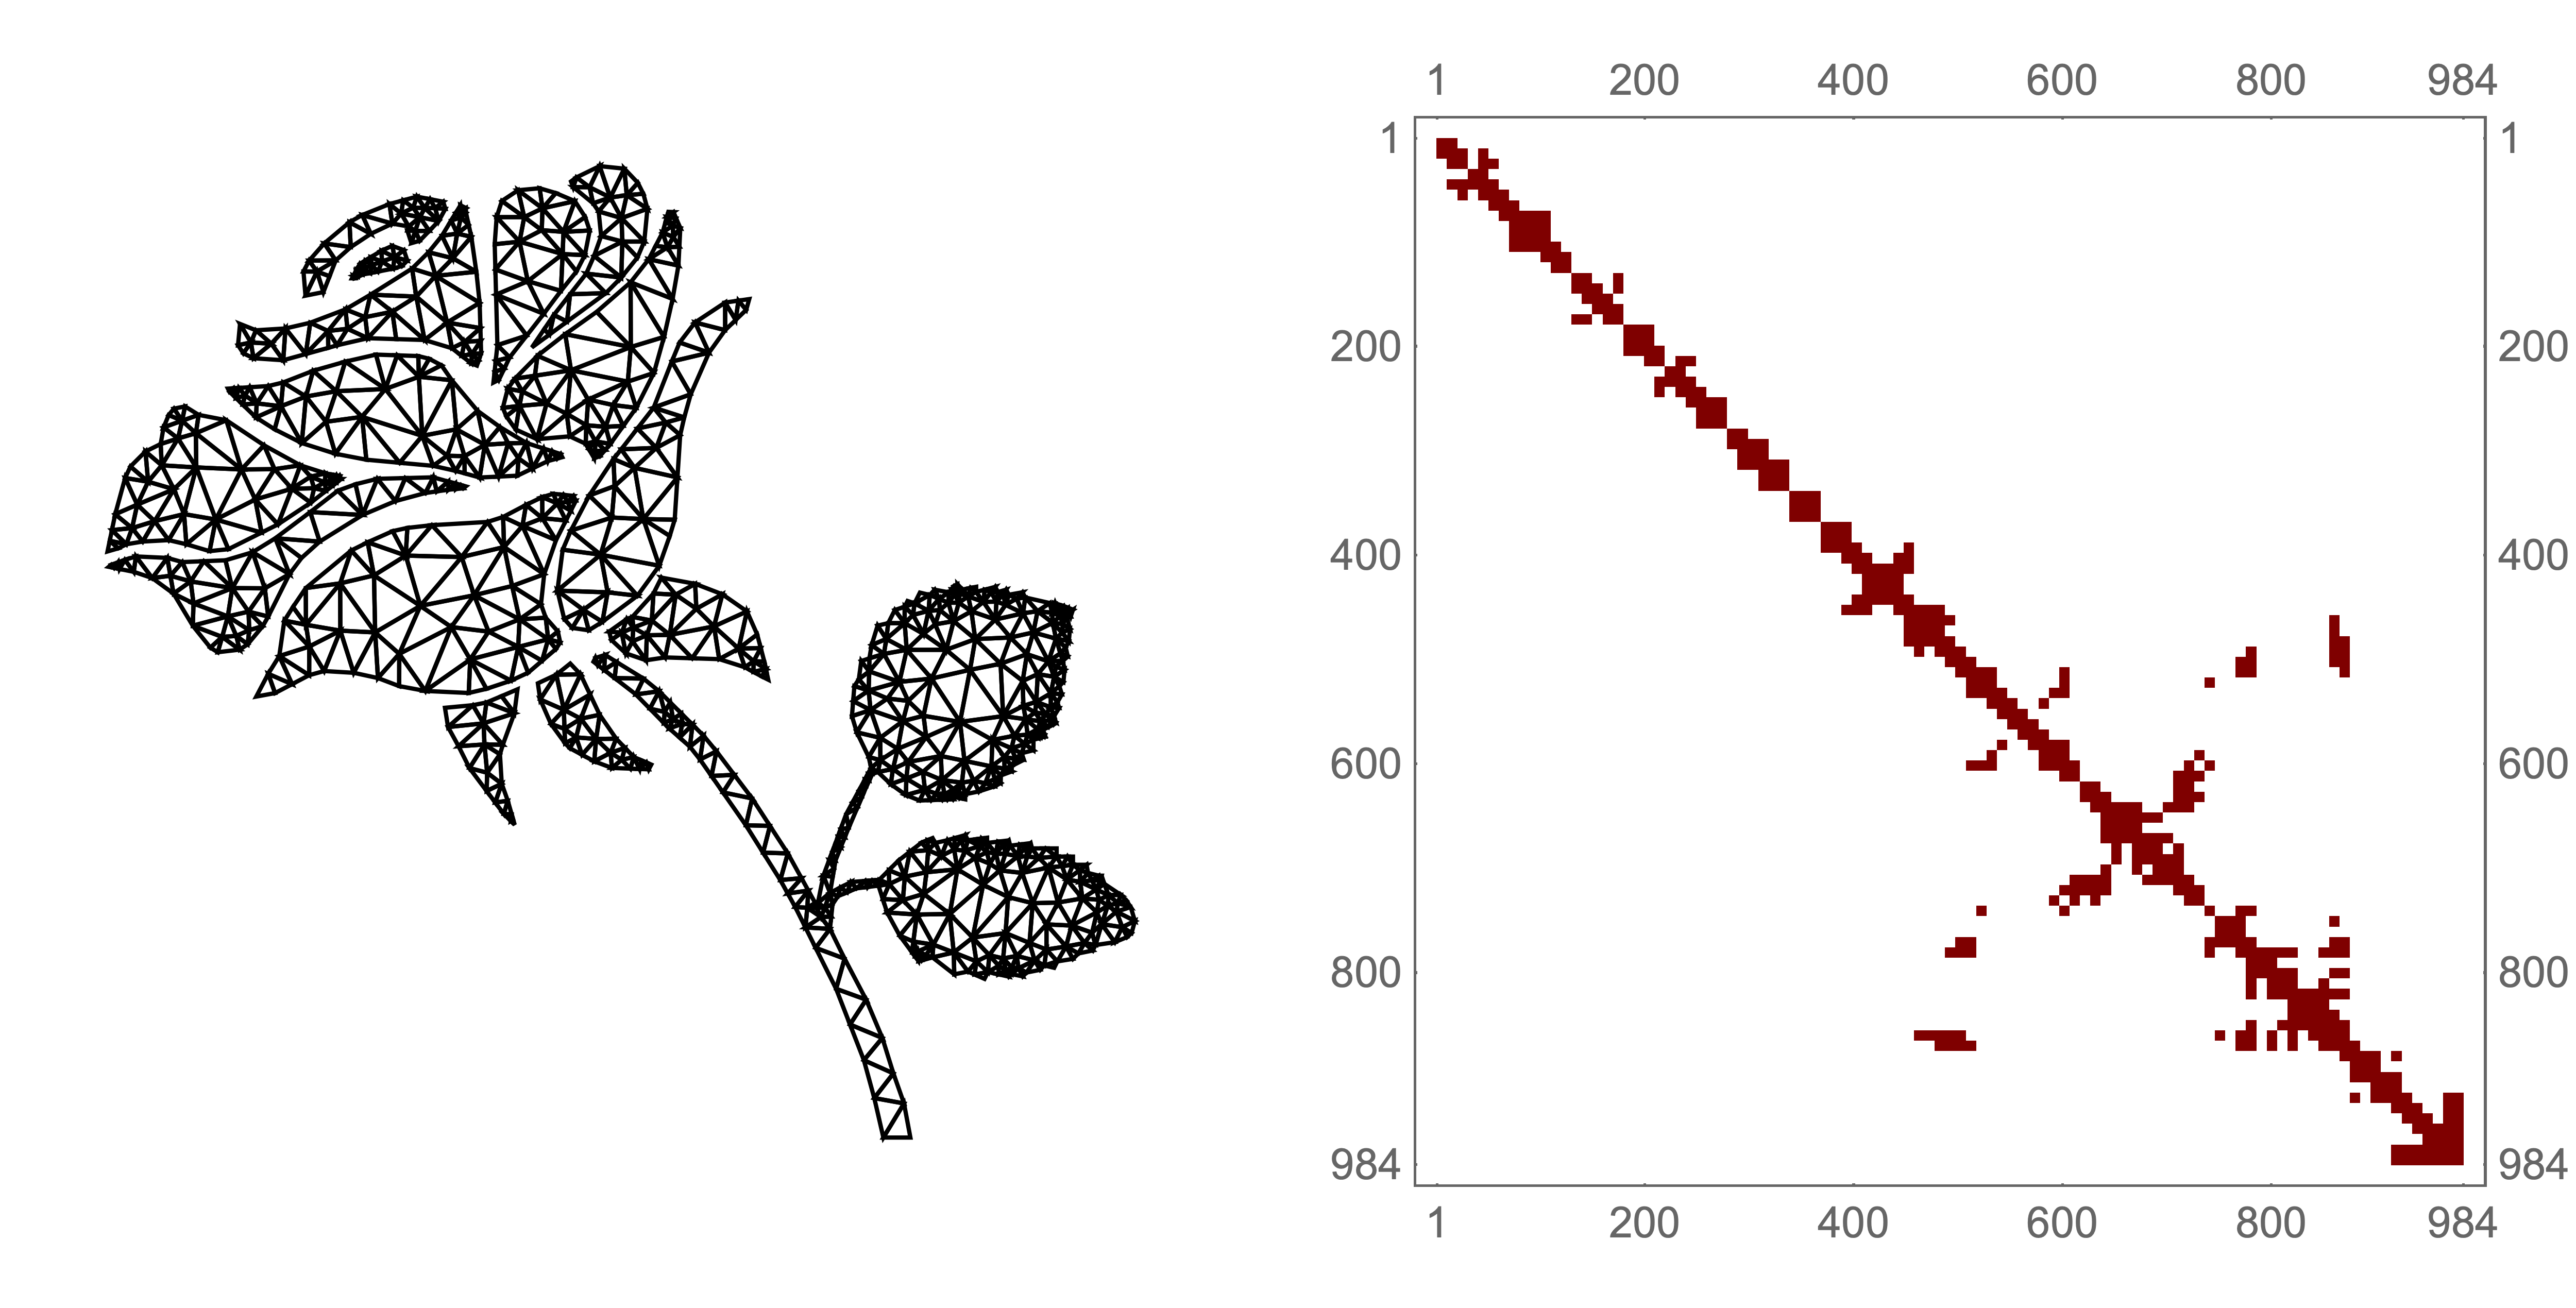
\includegraphics[width=2.5in]{meshmatrix.png}
        \end{center}
    \end{frame}

    \begin{frame}{Solvers}
        \begin{itemize}
            \item Linear FEM:\\
            Sparse linear systems solved with {\verb!scipy.linalg.sparse.spsolve}\footnote{Wrapper for SuperLU 4.0 (LU decomposition)}
            \item Non Linear FEM:
            Sparse non linear systems solved with {\verb!scipy.optimize.fsolve}\footnote{Wrapper for MINIPACK hybrj (Newton's Method + Gradient Descent)}.
            Jacobian is analytically computed to speed up the solver.
        \end{itemize}
        \begin{center}
            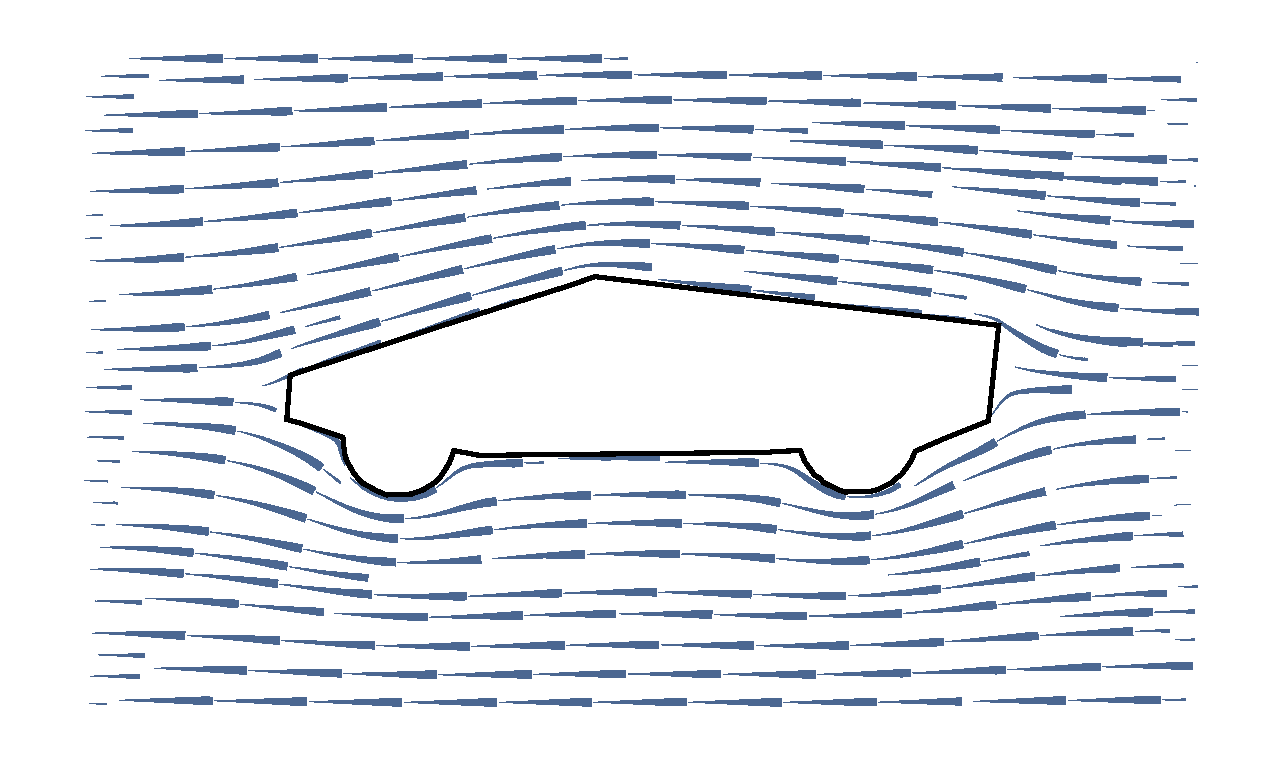
\includegraphics[width=3in]{cybercar.pdf}
        \end{center}
    \end{frame}

    \begin{frame}{Appendix: Mesh Generation and Format}
        \begin{itemize}
            \item Meshes are generated using the Mathematica 12 mesh generator
            \item Exported as:\\ list of coordinates [$x$, $y$]$^v$ \\list of mesh elements [$v_1$, $v_2$, $v_3$, marker]$^{e}$ \\list of boundary elements [$v_1$, $v_2$, marker]$^{be}$
        \end{itemize}


        \begin{figure}
            \centering
            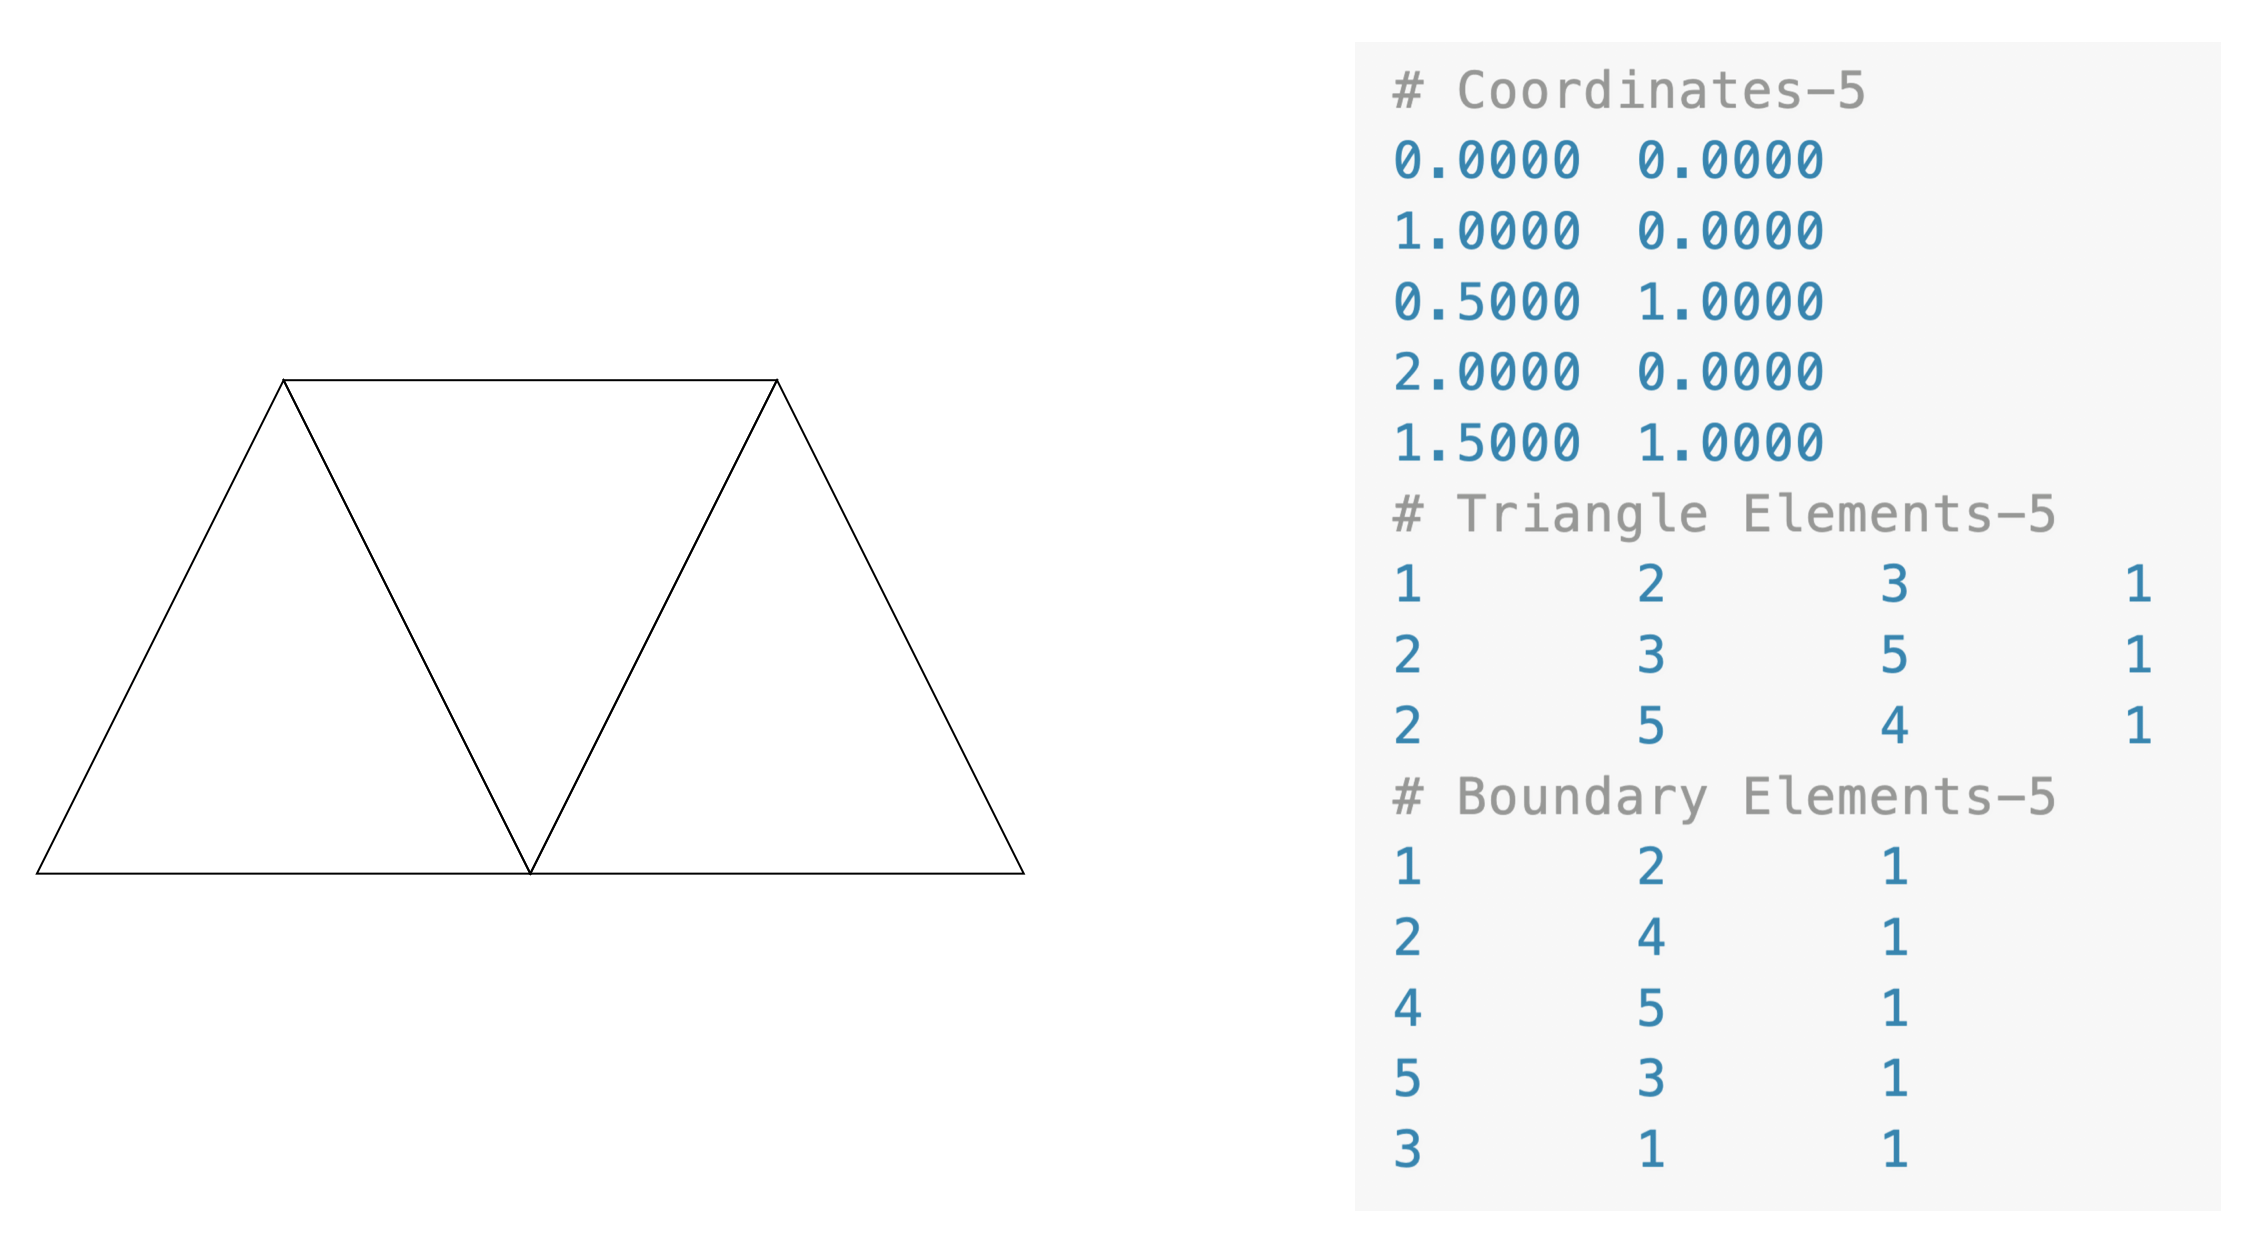
\includegraphics[width=3.5in]{meshdemo.png}
        \end{figure}
    \end{frame}
    \begin{frame}[fragile]{Appendix: Matrix Assembly}

        Global stiffness matrix assembly code for reference
        {\small
        \begin{verbatim}
    [(element[i], element[j], shp_fn.stiffness_matrix[i, j]
        * alpha(marker)) for i in range(3) for j in range(3)
        for element, shp_fn, marker in
        zip(elements, shp_fns, markers)]
        \end{verbatim}}
        List of all (row, col, val) tuples, overlapping values are summed.
    \end{frame}
    \begin{frame}[fragile]{Appendix: Gradient of $\alpha$}
        Given a function $\alpha(\|\nabla\phi\|)$ where
        \[\norm{\nabla\phi}=\norm{\left(\pdv{\vec{N}}{x}, \pdv{\vec{N}}{y} \right)^{\text{T}}\cdot \left(
        \begin{array}{c}
            \phi _i \\
            \phi _j \\
            \phi _k \\
        \end{array}
        \right)}\]
        \[\nabla\alpha=\frac{\alpha'(\norm{\nabla\phi})}{\norm{\nabla\phi}}
        \left(\pdv{\vec{N}}{x}\cdot\left(\pdv{\vec{N}}{x}\right)^{\text{T}}+
        \pdv{\vec{N}}{y}\cdot\left(\pdv{\vec{N}}{y}\right)^{\text{T}}\right)\cdot \left(
        \begin{array}{c}
            \phi _i \\
            \phi _j \\
            \phi _k \\
        \end{array}
        \right)\]
    \end{frame}
\end{document}
